\documentclass[tikz, border=20pt]{standalone}
\usepackage{graphicx} % Required for \scalebox
\usepackage{amsmath}  % Required for \boldsymbol

% Define bold, friendly, "nursery" colors
\definecolor{popred}{HTML}{FF477E}
\definecolor{popyellow}{HTML}{FFD166}
\definecolor{popgreen}{HTML}{06D6A0}
\definecolor{popblue}{HTML}{118AB2}
\definecolor{poppurple}{HTML}{7209B7}
\definecolor{popdark}{HTML}{073B4C}

\begin{document}
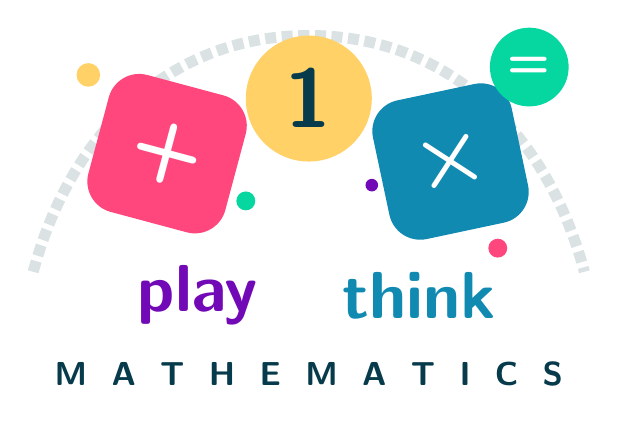
\begin{tikzpicture}[
  font=\sffamily,
  shapebox/.style={rounded corners=4mm, text=white, minimum size=1.8cm, align=center},
  shapecircle/.style={circle, text=white, minimum size=1.6cm, align=center}
]

% Playful dotted swoosh in the background
\draw[popdark!15, line width=4pt, dotted] 
(-3.5, 0.5) to[out=75, in=180] (0, 3.5) to[out=0, in=105] (3.5, 0.5);

% Tilted educational blocks/shapes
% Red Plus Block
\node[shapebox, fill=popred, rotate=-15] at (-1.8, 2.0) {\scalebox{3}{\textbf{+}}};

% Yellow Number Circle
\node[shapecircle, fill=popyellow, text=popdark] at (0, 2.7) {\scalebox{3}{\textbf{1}}};

% Blue Multiplication Block
\node[shapebox, fill=popblue, rotate=12] at (1.8, 1.9) {\scalebox{3}{$\boldsymbol{\times}$}};

% Little Green Equals Bubble
\node[shapecircle, fill=popgreen, minimum size=1cm] at (2.8, 3.1) {\scalebox{1.8}{\textbf{=}}};

% Main Brand Text: "play" and "think"
\node[text=poppurple] at (-1.4, 0.2) {\scalebox{2.4}{\textbf{play}}};
\node[text=popblue] at (1.4, 0.2) {\scalebox{2.4}{\textbf{think}}};

% Subtitle: "mathematics" spaced out for a clean foundation
\node[text=popdark] at (0, -0.8) {\scalebox{1.2}{\textbf{M \ A \ T \ H \ E \ M \ A \ T \ I \ C \ S}}};

% Fun decorative confetti dots
\fill[popyellow] (-2.8, 3.0) circle (0.15);
\fill[popgreen] (-0.8, 1.4) circle (0.12);
\fill[popred] (2.4, 0.8) circle (0.12);
\fill[poppurple] (0.8, 1.6) circle (0.08);

\end{tikzpicture}
\end{document}